%%%%%%%%%%%%%%%%%%%%%%%%
% Sample use of the infthesis class to prepare an MSc thesis.
% This can be used as a template to produce your own thesis.
% Date: June 2019
%
%
% The first line specifies style options for taught MSc.
% You should add a final option specifying your degree.
% *Do not* change or add any other options.
%
% So, pick one of the following:
% \documentclass[msc,deptreport,adi]{infthesis}     % Adv Design Inf
% \documentclass[msc,deptreport,ai]{infthesis}      % AI
% \documentclass[msc,deptreport,cogsci]{infthesis}  % Cognitive Sci
% \documentclass[msc,deptreport,cs]{infthesis}      % Computer Sci
% \documentclass[msc,deptreport,cyber]{infthesis}   % Cyber Sec
% \documentclass[msc,deptreport,datasci]{infthesis} % Data Sci
% \documentclass[msc,deptreport,di]{infthesis}      % Design Inf
% \documentclass[msc,deptreport,inf]{infthesis}     % Informatics
%%%%%%%%%%%%%%%%%%%%%%%%

\documentclass[mphil,deptreport,ai]{infthesis} % Do not change except to add your degree (see above).
\usepackage[final]{pdfpages}

\begin{document}
\begin{preliminary}

\title{Spiking neural network model construction, inference, analysis and application}

\author{William Peer Berg}

\abstract{
%   Lorem ipsum. More computational power. More data, and higher res. data available. Modelling may (1) explain aspects about recorded site(s), and (2) generate hypotheses that may be tested with in vivo recording.
%   However, inference of high-dimensional biologically realistic (to some extent) models NP-hard, computationally costly, does not scale well with growing resolution due to dimensionality and cost, and not automated. Often experts are required to make an effort at hand-engineering models for particular data. As such, model inference of biologically realistic/plausible models is a highly challenging task, which if more automated might be of great benefit to the field of computational neuroscience.
%   Looking to machine learning and the success in applying gradient-based optimisation to tackle high-dimensional modelling problems, we here investigate the potential of applying this to the class of spiking neural network models. Further, we look at statistical assessment methods, and application of outlined methodology both to synthetically generated as well as biologically recorded in vivo data.
%   In sum, our results show that models may capture higher-order statistics of recorded nuclei, and that using some parallelisation tricks, we may decrease the computational cost to some extent. However, the lower bound on computational complexity still makes it challenging to apply the outlined methodology to very rich (i.e. high number of recorded nuclei) data sets.

% ======== Should be rewritten after main text completed. ============
Computational models are used to try and explain observed data.
By implementing models that replicate observed data, the model itself may explain why and how the modelled system behaves as it does, and what its function is.
However, in order to be able to propose that the behaviour and functioning indeed arises due to mechanisms and dynamics similar to those in the model, the parallel between model properties and dynamics and in our case the brain and recorded nuclei needs to be firmly established.
These are usually established by design, and verified by statistical comparisons over different metrics.
However, to this day, constructing biologically interpretable and realistic models remains highly challenging, with no robust data driven approach working for other than very small networks.
While there is significant ongoing research efforts in bridging data driven approaches with computational modelling, this remains an unsolved task for neuron-level resolution spiking neural networks with a scalable methodology.
Currently, the most promising algorithm involves approximate Bayesian computation by training a deep neural network to approximate the posterior of the output (here spike trains) over the model parameters as the prior, and using simulation-based inference in order to generate samples, i.e. to simulate spike trains given a prior.
As the reader may note from this, the approach does not scale well - but it does maintain a full posterior over the parameters, as they are sampled altogether.
% SNNs biologically realistic models. 
Do we have the tools for SNN parameter inference, instead of rigorous and tedious hand-engineering?
ML advances: GBO.
SNNs differ from RNNs in a fundamental/crucial way. Show via parameter landscape and loss functions.
However, can find frontier(s).
SNN variants and applicability of GBO (only NLIF thus far, but still local minima).
To some extent GIF; frontier.
Same for GLIF versions??
Input scheme. Param landscape plots.
Loss functions.
PyTorch (+batching)

ABC, (EA; e.g. NGO)

Albeit GT off for the above, comparison wrt NMF.
Hand-engineered case and full analysis with NMF and LDA.

In conclusion...

BONUS (if time): Fitting to sleep data, with small sleep regul PPT/LDT lit rev first?

BONUS2: Append Izhikevich paper and place in context.

BONUS3: ?
}

\maketitle

\section*{Acknowledgements}

I would like to thank my supervisory team for offering their advice throughout my research.
I would also like to thank members of my lab group whom offered invaluable support and advice on everything from my project work to mastering stress and finding a flat in Edinburgh.
I also sincerely appreciated input relating to mathematics and philosophy from two special friends in Ediburgh whom are outside of my lab group - you know who you are.
Lastly, I would like to sincerely thank the head of our collaborative lab at the University of Strathclyde whom gave me access to in vivo data from the brainstem that was analysed wrt sleep regulation. It was truly inspiring and exciting to be able to see their experimental lab from early on in my project work.

% Nina.
% Matthias.
% Shuzo.
% Luke.
% Patricia.
% Etienne.

\tableofcontents
\end{preliminary}


\chapter{Introduction}


% The report then contains a bibliography and any appendices, which may go beyond
% page~40. The appendices are only for any supporting material that's important to
% go on record. However, you cannot assume markers of dissertations will read them.

% Citations (such as \cite{P1} or \cite{P2}) can be generated using
% \texttt{BibTeX}. For more advanced usage, the \texttt{natbib} package is
% recommended. You could also consider the newer \texttt{biblatex} system.

% You may not change the dissertation format (e.g., reduce the font
% size, change the margins, or reduce the line spacing from the default
% 1.5 spacing). Over length or incorrectly-formatted dissertations will
% not be accepted and you would have to modify your dissertation and
% resubmit.  You cannot assume we will check your submission before the
% final deadline and if it requires resubmission after the deadline to
% conform to the page and style requirements you will be subject to the
% usual late penalties based on your final submission time.

% MPhil:
% One who strives towards a goal to prove themselves, may suffer along the way.
% One who strives towards a goal as a means of self-expression, may enjoy the way.


Spiking neural networks (SNNs) contain variables that represent biological properties such as membrane potential, temporal signature, and potentially ion channel dynamics. Their definition results in membrane voltage dynamics resembling that of biological neurons, including the release of action potentials upon reaching a certain membrane potential.
Due largely to the biological plausibility of this class of neural network models, they are appealing to study in computational neuroscience, as they may trail biology to a greater extent than the feed-forward networks as often seen in the machine learning domain.
However, training SNNs is yet of limited success, and model inference also faces a number of challenges due to the temporal constraints introduced by SNNs, as well as the increased complexity of this model class.
We here revisit the state-of-the art for inferring SNN models using both surrogate gradient based optimisation and some of the most prominent spike metrics, as well as deep neural network amortized learning and approximate Bayesian computation (ABC), and compare how these approaches may be employed for SNN inference. Further, we hypothesise that recent ML techniques may be leveraged for successful and efficient model inference using surrogate gradient descent.
We find that while ABC may be successful for population-level models, as has been shown recently in the literature, its algorithmic and computational complexity and cost thereof limits the methodology to a low number of nodes, particularly for more high-dimensional leaky integrate-and-fire (LIF) model extensions.
However, using a surrogate gradient approach, we find that model inference for larger networks is made possible. 
Since it would greatly help with SNN model construction if automatic inference based on various data became possible and available to the research community, this has been one of my primary research goals.
Further, as usual, more and more data, and data of a higher resolution, is becoming available from neural brain recordings, only increasing the potential benefits of developing a scalable approach for model inference.
We perform model inference using a set of LIF-extensions, leading up to the GLIF model using (both) synthetic (and biological) data, and demonstrate that higher order statistics may be captured (to some extent) even when performing neuron-level model inference over a mixed neuron-type network.
% This may advance research on SNN inference, and also demonstrates how modern ML frameworks as well as techniques may be leveraged to this end.
However, we observe that it is highly problematic to aim for retrieving ground-truth parameters in SNN models. A large part of the work presented in this thesis will revolve around why SNNs do not lend themselves as well as feedforward neural networks as within deep learning, even though they also implement a type of recurrence using recurrent units with memory, in addition to potential recurrent connectedness.
To try and give an intuition about why this is; if we think about deep neural networks (DNNs) in the machine learning (ML) domain - these may approximate arbitrary data well, given that they are universal function approximators. However, this requires that the data is of such a format that it may be represented and captured by a function which the network learns by spatial representation and transformation.
However, in the domain of SNNs, we introduce several new crucial properties, which results in distinct model dynamics. Each neuron now has a state, which depends on its previous state, and the behaviour is modelled typically as a system of ordinary differential equations (ODEs), containing parameters representing the membrane potential, membrane time constant relating to a refractory period, transmitter interaction, and other biological properties. 
While this makes the model biologically interpretable with direct parallels between parameters and biological and cellular counterparts, it also changes the entire system's behaviour.
The system now has activity inedpendently of input perturbation. The transformation of an input signal is no longer deterministic in the sense that it will result in one given output given a set of initial model parameters - it now depends on the current system's state, which again depends on the previous state.
As such, gradients calculated in a manner similar to that of for DNNs in ML will also depend on the system's and neurons' state, greatly increasing complexity.
In a way, one may still maintain the parallel to backpropagation through time for DNNs - however, there is a crucial difference in that a neuron's output is now of a much more binary nature; a spike or no spike, and in that the time series evolution of spikes, whilst potentially encoding much more information, now is a series of spike evolving over time, and thus the target signal cannot be regarded in the same way as in DNNs.
This being said, I believe like noted by other authors such as \cite{Sindaci2018StatisticalFunction} that researchers are looking for a connection between the field of machine learning and computational neuroscience, the former having had its subfield of DNNs created based on inspiration from the brain, but now in a reverse way in which we may leverage the advances from the domain of ML in model construction.
Even though we are not there yet, I believe the search for a connection here may both be highly beneficial for the community, and spawn a new sub-field of dynamical systems modelling using inference in computational neuroscience.

My main findings, although included throughout in the rest of my thesis, may be summarised as following:
\subsection{SNNs are hard to optimise}
I am starting to believe that they’re in fact not possible to optimise, due to the parameter landscape, which results from the temporal nature of the target signal.
In DNNs, we only consider approximating a spatial transformation over the input data. Not only does this allow for higher parallelisation of the training algorithm, but it may also greatly constrain the parameter landscape in the sense that it does not depend on the past activity of the network itself, which vastly increases both the complexity and stochasticity of parameter inference. 
One way to ameliorate this is to eliminate some of the stochasticity by making the neurons non-leaky. Since we may computationally set the system’s initial conditions and random seed, the following deterministic computations have little to no fluctuations, and with no leakage, gradient propagation may be computed exactly according to the error signal.

\subsection{Another issue of SNNs is the binary output signal}
One way of addressing this issue is by incorporating the signal below spike-threshold, i.e. the membrane potential, and have this generate a signal inside of an active zone, such as when the potential is above 0. This is not entirely biologically unrealistic, …, and it offers the advantage of a continuous signal centred around potential (no pun intended) spike pulses, or action potentials. Note that it also provides a gradient signal for spike generation even when the potential may be below threshold, still making the excitation visible to the optimiser.
This bears some resemblance to loss metrics such as the van Rossum distance, in which each spike pulse is convolved with an exponentially decaying kernel, such that we may operate over a smoother signal. However, this signal transformation transforms each spike pulse the same, rendering the sub-threshold gating synapse model a more fine-grained candidate, since it contains richer differentiable information, and not just spike-time information.

\subsection{Multiple local minima - no well-defined global optimum}
Even when addressing the issues above with the proposed approaches, and even if fixing all model parameters but the weight matrices, there are multiple weight configurations that may result in very similar behaviour and outputs.
As noted by other researchers in the DNN as well as SNN literature (...) the initial configuration has a large effect on the resulting inferred weights and/or model. This holds particularly true for SNNs, where the previous model state also has an effect on the future state, and the model neurons may be brought to exert different modes of behaviour, depending on the previous and current input and state.

\subsection{Hand-engineered models may be qualitatively similar to local minima}
By hand-engineering models it is possible to attain qualitative patterns and behaviour, which has been a common practice in the field of comp neuro - however, this may not be satisfactory for attaining higher-order statistics, and requires a large amount of resources. Therefore, model inference may likely be a better option. 
The above however indicates that GLMs may be the best we can do in this regard (wrt spike trains), and demonstrates a need for advancing SNN inference.
The way going forward?
Amortised learning provides a posterior over the parameters.
However, it quickly becomes intractable due to the high complexity of models.
Surrogate or exact gradient approaches are difficult due to aforementioned issues, and most likely do not settle into a stable configuration, as well as stay in planes of local minima.
These findings suggest that the best we can currently do is using approximate Bayesian approaches, which not only lets us infer a posterior over all of the parameters, but also provides a measure of certainty around the parameters.

Temmporary conclusion:
If this approach is intractable for the case we’re looking at, the best we may do is either to use other information theoretic approaches to assess whichever aspect it is that we are interested in, including potentially to hand-engineer and rigorously test a proposed model.

% =======================================================
\chapter{Background: Biologically plausible computational modeling}

Various SNN models

\cite{Taherkhani2020} learning in SNNs

Mackelab meso paper: Only rate based at first.
NN 2020 review: Loses out on temporal information.
NMF: Spatiotemporal decomposition - thus rate based should not be able to infer spatial activation coefficients. However, encode populations into SGD, and rate based may? 
Topological averaging.
Search using micro-model directly? Data set requirements? Spike trains - rate per node and binom dist.?


\section{Fundamental differences between SNNs and spike train PDF models}


\section{The link to recurrent neural networks (RNNs)}


\section{Bayesian approaches}

\subsection{MCMC sampling}
\cite{Rene2020} "special case" i.e. mesoscopic-microscopic inference using first ABC (or GD?) on pop. level and then MCMC sampling for full approx. posterior?

“To understand how rich dynamics emerge in neural populations, we require models which exhibit a wide range of dynamics while remaining interpretable in terms of con- nectivity and single-neuron dynamics. However, it has been challenging to fit such mechanistic spiking networks at the single neuron scale to empirical population data. To close this gap, we propose to fit such data at a meso scale, using a mechanistic but low-dimensional and hence statistically tractable model.”
Argue that instead of making the reduction to a population-level model, we may instead make the dimensionality reduction for the parameters.
There exists work on fitting GLIF parameters to physiological data. 
Also, inferring weights with fixed parameters is possible using GD, given data.
This could mean that we could, given the correct neuron classes, infer a topology or the connectivity of a site recorded from!
Parameters may be inferred prior to the weights using an appropriate procedure.
However, in the Rene-paper they use aggregate population activity, or spike histories, and derive the likelihood for the parameters. Can be used to either optimise, or do Bayesian inference.
They conclude that population inference impact and improve the accuracy in single-neuron parameter inference.

The René paper assumed known input when inferring models. They also generated data with sine-modulated input.
They also made a quasi-renewal approximation, and assumed independence between neurons in each time bin.


\subsection{Amortised learning with DNNs}
\cite{Lueckmann2018} amortised learning and ABC using DNNs.

SNPE

\section{Evolutionary algorithms}
I recall back to conferences talking about inferring complex, deep networks, which is a field where evolutionary algorithms (EAs) still are competitive and fruitful.
In short, when EAs are fruitful, this often means the search space is so vast that gradient-based approaches will not converge.

let's forget about casting the spike trains into a euclidean space, and propagating gradients. let's relax this to defined operations where there is a cost assigned to each operation, such that there is a minimal distance between two spike trains. this should let us define operations for moving single spikes, and shifting spikes. however, in my case there is uncertainty involved, so we should define operations for matching motifs instead. this makes it unclear for polynomial-time DP for calculating the distance. i can do pattern identification according to pre-defined rules, which will be exponential over a constant bound such that for longer time-intervals, a greedy comparison should be polynomial.
if we assume that parts cannot cross in graph-matching, however, it becomes polynomial for the full distance-calculation (for larger intervals)

sin (f(s)) + cos (g(s)) ?
where f(s) = D\^spike[q, k]
and g(s) = D\^interval[q, k]
assume same labels?


--> However, does not converge well.


\section{Analysing SNNs}

Not straightforward how to analyse... Should this be in background or later?

\subsection{NMF}

\subsection{LDA}

\subsection{Generalised Linear Models}


\section{Models}

\subsection{LIF}

\subsection{Generalised leaky integrate-and-fire (GLIF)}

\subsection{Non-leaky integrate-and-fire (NLIF)}

\subsection{Izhikevich}

Replicated \cite{Oliveira2019} merely to show that the resulting rates could be formulated more or less as a linear function, resulting from subthreshold oscillations, and that the model is highly sensitive to its initial parameter values.
All modes of behaviour as observed in biology, however something needed to shift mode(s) of behaviour..
Parallels to SNN inference etc

\subsubsection{Poster: \textit{The effect of the recovery variable parameters on oscillating Izhikevich networks}}
\includepdf[pages=-]{files/berg_and_onken_uk_neural_computation_2019_poster.pdf}


\section{Loss metrics}

% ---------------------
\textbf{Something you can learn about network, but also should be specific to a spiking net
Want to find something only in SNN, but which is also identifiable
Don’t need to find exact same sync act., not same identities of neurons which participate, just general properties, in spite of unknown input activity}

Advantages of SNNs compared to rate based/mean field
Quantity
Model statistics exhibited regardless of configuration
Different inputs and generative model output variability

“Vector strength is the Fourier component of the spike sequence at the stimulus frequency normalized by the total number of spikes”

“It has been proposed that membrane time con- stant, spiking threshold, and the number of inputs per period are key parameters that determine the performance of a coincidence detector (Kempter et al. 1998)”
On temporal info coded by phase-locked spikes processed in higher-order centers in the brain

Precise firing sequence
“Inappropriate surrogate” - high-order gamma dist great number of chance patterns due to generating quasiperiodic spike trains. Poissonian more unrelated periodic spike trains
“Nonprecise time patterns” - interested in spike patterns (not one less precise peak in 3d corr M)

% (Analysis and interpretation of interval and count variability in (single neuron) neural spike trains
% Coefficient of variation (CV), trial-by trial count variability with the Fano factor (FF), estimation bias, …
% Variability on tens to hundreds of ms
% CV = SD(X)/E(X))

Can we detect statistics relating to state in data using more sophisticated rate measures when compared to straightforward mean binned rates per state? Could this be used further?

System. Spike train assumed to be distributed according to some distribution. Can invert and calculate probability and minimise. Fluctuation can for instance be regarded as due to “irregularity in time from a constant rate or regularly from a fluctuating rate”.
Metric measuring ISI variability rescaled locally in time can suggest which is more plausible.
When looking at more complex system this is less trivial..? MIght be used on higher-level such as neuron classes?

Need to go beyond renewal processes to capture different neuronal modes of behaviour, and spike train adaptation - serial correlations in ISIs is one such step
Hidden Markov processes, drawn from distribution relative to state
“Memory” in nesting the probability such that it depends on N preceding ISIs

Grün and Rotter, methods
Characteristics that are stable in spite of different inputs

Null hypothesis: Independence (spike trains)
stochastic spike train models, posits probabilistic model for timing of spikes, based on the spike history. Simplest such; Poisson process.
p(spike\_[t, t+dt]) ~~ Rdt, where R is the rate (for sufficiently small dt)
Point processes for several spike trains (networks and not just neurons); papers (ignored here)
% ---------------------


% =======================================================
\chapter{Work: The frontier of SNN inference}

In order to study how to infer spiking neural network models (SNNs) one needs several ingredients: (1) a definition of the entire system, (2) an implementation of it, (3) an algorithm for model inference where (1) and (2) are compatible with the algorithm, and (4) a way to measure and assess model performance, ideally compared with existing methodologies and models.

Research on SNNs using gradient-based optimisation is fairly limited, and includes approximate Bayesian computation for smaller models, conversion learning in which more traditional ANNs are transformed to simpler SNNs after training, or surrogate gradient descent, in which a surrogate signal over the model spikes, usually as a function over the membrane potential, is used in order to obtain a differentiable output that may be used to optimise the model's parameters over a given loss metric by backpropagating the error signal.
% Currently, the state-of-the-art methods are only partly successful in training a subset of SNN model parameters for smaller models.
With the goal of accelerating SNN inference research, I looked at the most prominent state-of-the-art methodologies for SNN inference, which may be divided into (1) gradient based optimisation (GBO), and (2) approximate Bayesian computation (ABC) \cite{Lueckmann2018, Rene2020, Cranmer2020a, Lueckmann2021}.
GBO enables leveraging recent ML advances from deep learning, and albeit biologically implausible as a learning rule, allows for in-place model inference training and inference. The computational cost of doing gradient based computation is also exponentially less than that of doing ABC, as this involves doing a Monte-Carlo sampling step \cite{Rene2020}.

Previously, Bayesian inference was intractable for SNN models due to their high-dimensional parameter-space, but recent advances in sequential neural estimation techniques, where a DNN is trained to estimate a prior using a relevant statistic, has allowed for much more efficient sampling using this amortised approach; sampling from the DNN to perform posterior parameter estimation.
Note however that this procedure still has a high cost, which does not scale well with an increase in the network size.
% references, brief summary and discussion of main references
Using a Bayesian approach, we may however estimate the posterior over the model parameters, given our approximation of the prior. This also yields a type of uncertainty estimate around the posteriors. Note however that the posterior will be skewed by the prior approximation, in our case given by sequential neural ratio estimation (SNRE) \cite{Lueckmann2021}.
 
Using a surrogate gradient approach, we may fit the parameters of the system by error minimisation using any differentiable loss function. Due to the constraint put forth by working with biological spike train data, which is a very widespread format in which there is a vast amount of data available, we cannot however make many assumptions about the input, unless the recording somehow also contains information about this signal. 
Therefore, we have to include the input in the model, by making assumptions about the network input, as well as to consider how it may greatly affect network behaviour during learning. As a rule of thumb, we want to have a signal which allows for the network to perform the task at hand, or to replicate the observed data, whilst being as biologically reasonable as possible.
We want to have input that puts the system in a realistic mode of behaviour, and allows us to optimise its parameters such that an informative signal is transformed in a meaningful way.
% As it is limited what we may assume about the input, loss metrics that put a high emphasis on the precise timing of spiking may in fact obscure the gradient signal by incorporating too much of the noise stemming from this signal.
% We therefore focus on metrics that are more rate-based, looking at intervals of spikes in order to include the temporal signatures to some extent.
% Using a timing-oriented metric over larger time bins may even result in divergence, due to variability between the hidden target data input, and the inferred model input. 




\section{My contribution: Implementing, differentiating and optimising different SNN models using different loss metrics}

Goals and questions or hypotheses
Novel method developed for advancing SNN inference by using gradient descent
Binary in nature, by implementing surrogate subthreshold spike signals, we may facilitate optimisation, improving optimisation performance for gradient descent.
We will retrieve a local minimum which is not approaching ground-truth in terms of model parameters, however, the model will capture the spike statistics to a greater extent than other models. As such, it may be used to evaluate the functional characteristics of the modeled nuclei.
The input is unknown.
% SBI approach for SNN inference; limitations. Test potential.
% Better for true parameter estimation. However,  posteriors are probability densities, and do not have direct access to full model configurations as such, and may suffer from not capturing full specific model configurations that capture as many higher-order spike statistics.
% GLMs as a baseline to have comparable results for NMF analysis
% Input transformation (?, avg. relative spiking per population ?)
% net(x\_forward)
% Output transformation (avg. v per pop.)
% Can transform spike-train to average population membrane potential
% Synapses with dg/dt ?
% self.g = torch.ones\_like(self.v)  for one conductance per neuron (for n synapses)

\subsection{Contribution: PyTorch}

... tricks, sequentiality etc

\subsection{Contribution: Batching and SNNs}

even though sequential constraint, each batch is parallelisable, effectively doing batch norm over batches in parallel.

\subsection{Contribution: Loss metrics comparison}

Tricky design, stochasticity, lots of considerations, as we shall see only frontier..


\subsubsection{van Rossum distance}
Hypothesis: Using the van rossum distance may guide search, allowing gradient-based methods to converge?

Using the van-rossum distance as a loss function for the spike trains, we get something more continuous, since the discrete spike train is convolved with a time-based kernel. This should make the gradients more informed via the loss function in larger search areas.

Main finding: 
"\textit{wandering gradients}" for vRD.

One thing is quantifying distances in terms of spike metrics.
Another is designing a metric that is well-defined for gradient-descent.
While the van Rossum metric describes the distance between two spike trains both in terms of rates and timing, due to its sensitivity to exact timing the gradient signal might be obscured for non-matching neurons, and more well-defined where the rates better match.

\section{Leaky integrate-and-fire (LIF)}

Currently, I’ve implemented a setup that fits an arbitrary model to spike train data. I have generated synthetic data using a LIF model, and am trying to fit a LIF population model to this (the simplest scenario I could think of).
When fixing most parameters, only trying to fit the population connectivity weights, it does not currently always converge. I am currently working on this.

Gradient-based methods prone to finding sub-optimal solutions, i.e. local minimas. This is an issue particularly for high-dimensional feature spaces. Thus, I am led to believe this will be an issue when trying to infer the model parameters of complex neural networks using spike trains.

%--------------------
LIF work log:
More nuanced
Very noisy gradients for unstable/chaotic generative model perturbation?
Dynamic R\_I in conjunction with frd might result in better convergence, due to constraining search space.
By using dynamic R\_I (linear constraint), this makes behaviour more stable, and so may allow for more calibration/optimisation of the other parameters.

vRD suddenly seems viable for more stable network behaviour. When model behaviour was more chaotic, frd was better. This makes sense, as gradient will not be well-defined for vRD when model is chaotic. Not necessarily for frd either, but this is more robust to noise.

Some artefacts LIF (more linear, easier to have whole-network spiking with too little inhibition / simpler neuron dynamics)

Initial conditions large effect on convergence

vRD performance OK with tau=100.0
frd better
In conjunction: still sometimes silent neurons. Potentially due to local minima of vRD for silent neurons, and obscured parameter-landscape due to noise and the nature of the vRD-metric. Not necessarily orthogonal to frd either, and as such may interfere with its gradient

Will have to look at vRD vs frd vs frd+vRD vs adaptive(frd+vRD) quantitatively for setups.

There seem to be many regions for which there is no “information gain” when moving along gradients, such as for silent neurons. Some parameters might not have their effect obscured or less pronounced due to the change of other parameters in parallel, too. This is the reason other authors have performed sequential parameter optimisation.

When constructing generative target models, we aimed for hand-engineering models entraining higher-order ensemble dynamics that were stable across different random seeds of model perturbation, such that we could test how well model inference would capture these statistics. To this end, we designed three populations of neurons, where each population had different neuron parameters, normally distributed around set means, with a standard deviation of 25 % around the population values for each neuron. 
In order to not generate spurious data, such as if the generative model is driven primarily by its input perturbation, or where it behaves otherwise chaotically, we tested that the hand-engineered models’ higher order statistics indeed occurred across different random seeds.

(To verify that the model would indeed be sensible for synthetic generation, we tested the stability of neuron rates across different random seeds. When a deviation lower than X was attained, we accepted the ensemble model as a generative model suitable for data generation in order to test our framework.)
Note that this deviation test is only to determine that the model doesn’t behave chaotically, and does not fire spuriously, in which case optimisation would be like fitting to noise, which should not converge.



\section{"Cortical microcolumn"-inspired stochastic population integrate-and-fire models}

microGIF


\subsection{Stochasticity and SNNs}

\subsection{Contribution: microGIF work}

\subsection{GLIF neurons}

Can be highly parameter-sensitive and result in completely different mode of neuronal behaviour

GD: 
N=3
LIF\_R, frd (SGD) looks good, albeit with mostly straight parameter trajectories
LIF\_R, vrd (SGD) OK
LIF\_R, rate+pcc (SGD) OK/good
LIF\_R\_ASC, frd, good
LIF\_R\_ASC, vrd, OK
LIF\_R\_ASC, rate+pcc, good
LIF (noisy target), frd, noisy OK
LIF (noisy target), vrd, not satisfactory/OK-
LIF (noisy target), rate+pcc, noisy OK
LIF\_weights\_only, frd, noisy very low loss, somewhat trailing train/test
LIF\_weight\_only, vrd, noisy higher loss, closely trailing train/test
LIF\_weights\_only, rate+pcc, fairly low loss, somewhat more trailing train/test
LIF\_fixed\_weights, frd, noisy medium/low loss
GLIF, frd, somewhat noisy and trailing low loss, looks good, nonlinear param trajectories

N=10/12: Breaks down(?), or wanders along frontiers (wandering gradients in SNNs)


\subsection{Model input perturbation and formulation}

Task: Model site from which spikes have been recorded and decoded. Issue: We don’t have the input to the site. Options: Auto-encode temporal evolution of spike train, or infer model to produce outputs when noise-driven. Question: Is this at all attainable?

Learning methods:
BP, BPTT, Surrogate gradient (what we’re doing), soft-threshold (very similar to what we’re doing, but not in-place), STDP (has similarities, but not what we’re doing - more suitable to local and temporal learning?)

One finding is that we can infer a LIF SNN capturing higher-order statistics with a noise-driven setup (during inference). Using more temporally oriented loss functions quickly becomes problematic due to the input-noise, however. Can we show this analytically or empirically somehow for more complex models?
Another scheme: Predict next input given previous - (learn patterns from the information we have) then predict when perturbing with noise. Would also allow for hand-engineering input with different qualities (inspired by vigilance/sleep state), and test whether functional ensembles resemble those observed during these states in vivo.

Given the learning algorithms that we have available, how detailed spiking models may we infer by using common data sets? More specifically, can we increase the level of detail and level of higher-order statistics captured in a model by also inferring internal neuron variables by using gradient-based optimization? Is this possible by only using a one-dimensional target signal, such as spike trains? Does more detailed neuron models than LIF models enable capturing a higher level of detail and statistics, through allowing a wider array of model behaviour? Can we fit these models in a noise-driven scheme, such that the approach may be used on real-world data? If not, what are our alternative approaches? Could we for instance fit to output data given previous output data, i.e. similar to auto-regression? If so, would this enable us to predict output under different brain states?
Model inference should be compared to common statistical models, including GLMs, Gaussian mixture models, and Poisson models.


Method assumes access to observed neural activities and external input.
René et al. (2019/20) paper:
“The method we present assumes that the model to be inferred can be expressed as a
set of stochastic equations and that we have access to time series for both the observed (and possibly aggregated) neural activities and external input”


\subsubsection{Poisson input}

\subsubsection{Cyclic input}

\subsubsection{Cyclic input and white noise}

\subsection{Multi-layer versus single-layer SNNs}

Multi-layer net crucial for non-linear function approximation! We have not had this. If we only wish to capture the spike statistics, then a multi-layer version training on the next spike given the previous could perform better than the current single-layer noise-input to spike output?
What we have tried is instantaneous reactivity given noise-input. Is this not largely spatially oriented? To include a more temporal orientation, we may need to redesign the setup.

Auto-encoding task of own readout would make sense. However, we only have the binary spike output, and not continuous membrane potential



% =======================================================
\chapter{Gradient-descent based LIF SNN inference}
\section{Poster: \textit{Spiking Network Inference Using Gradient Based Optimisation}}
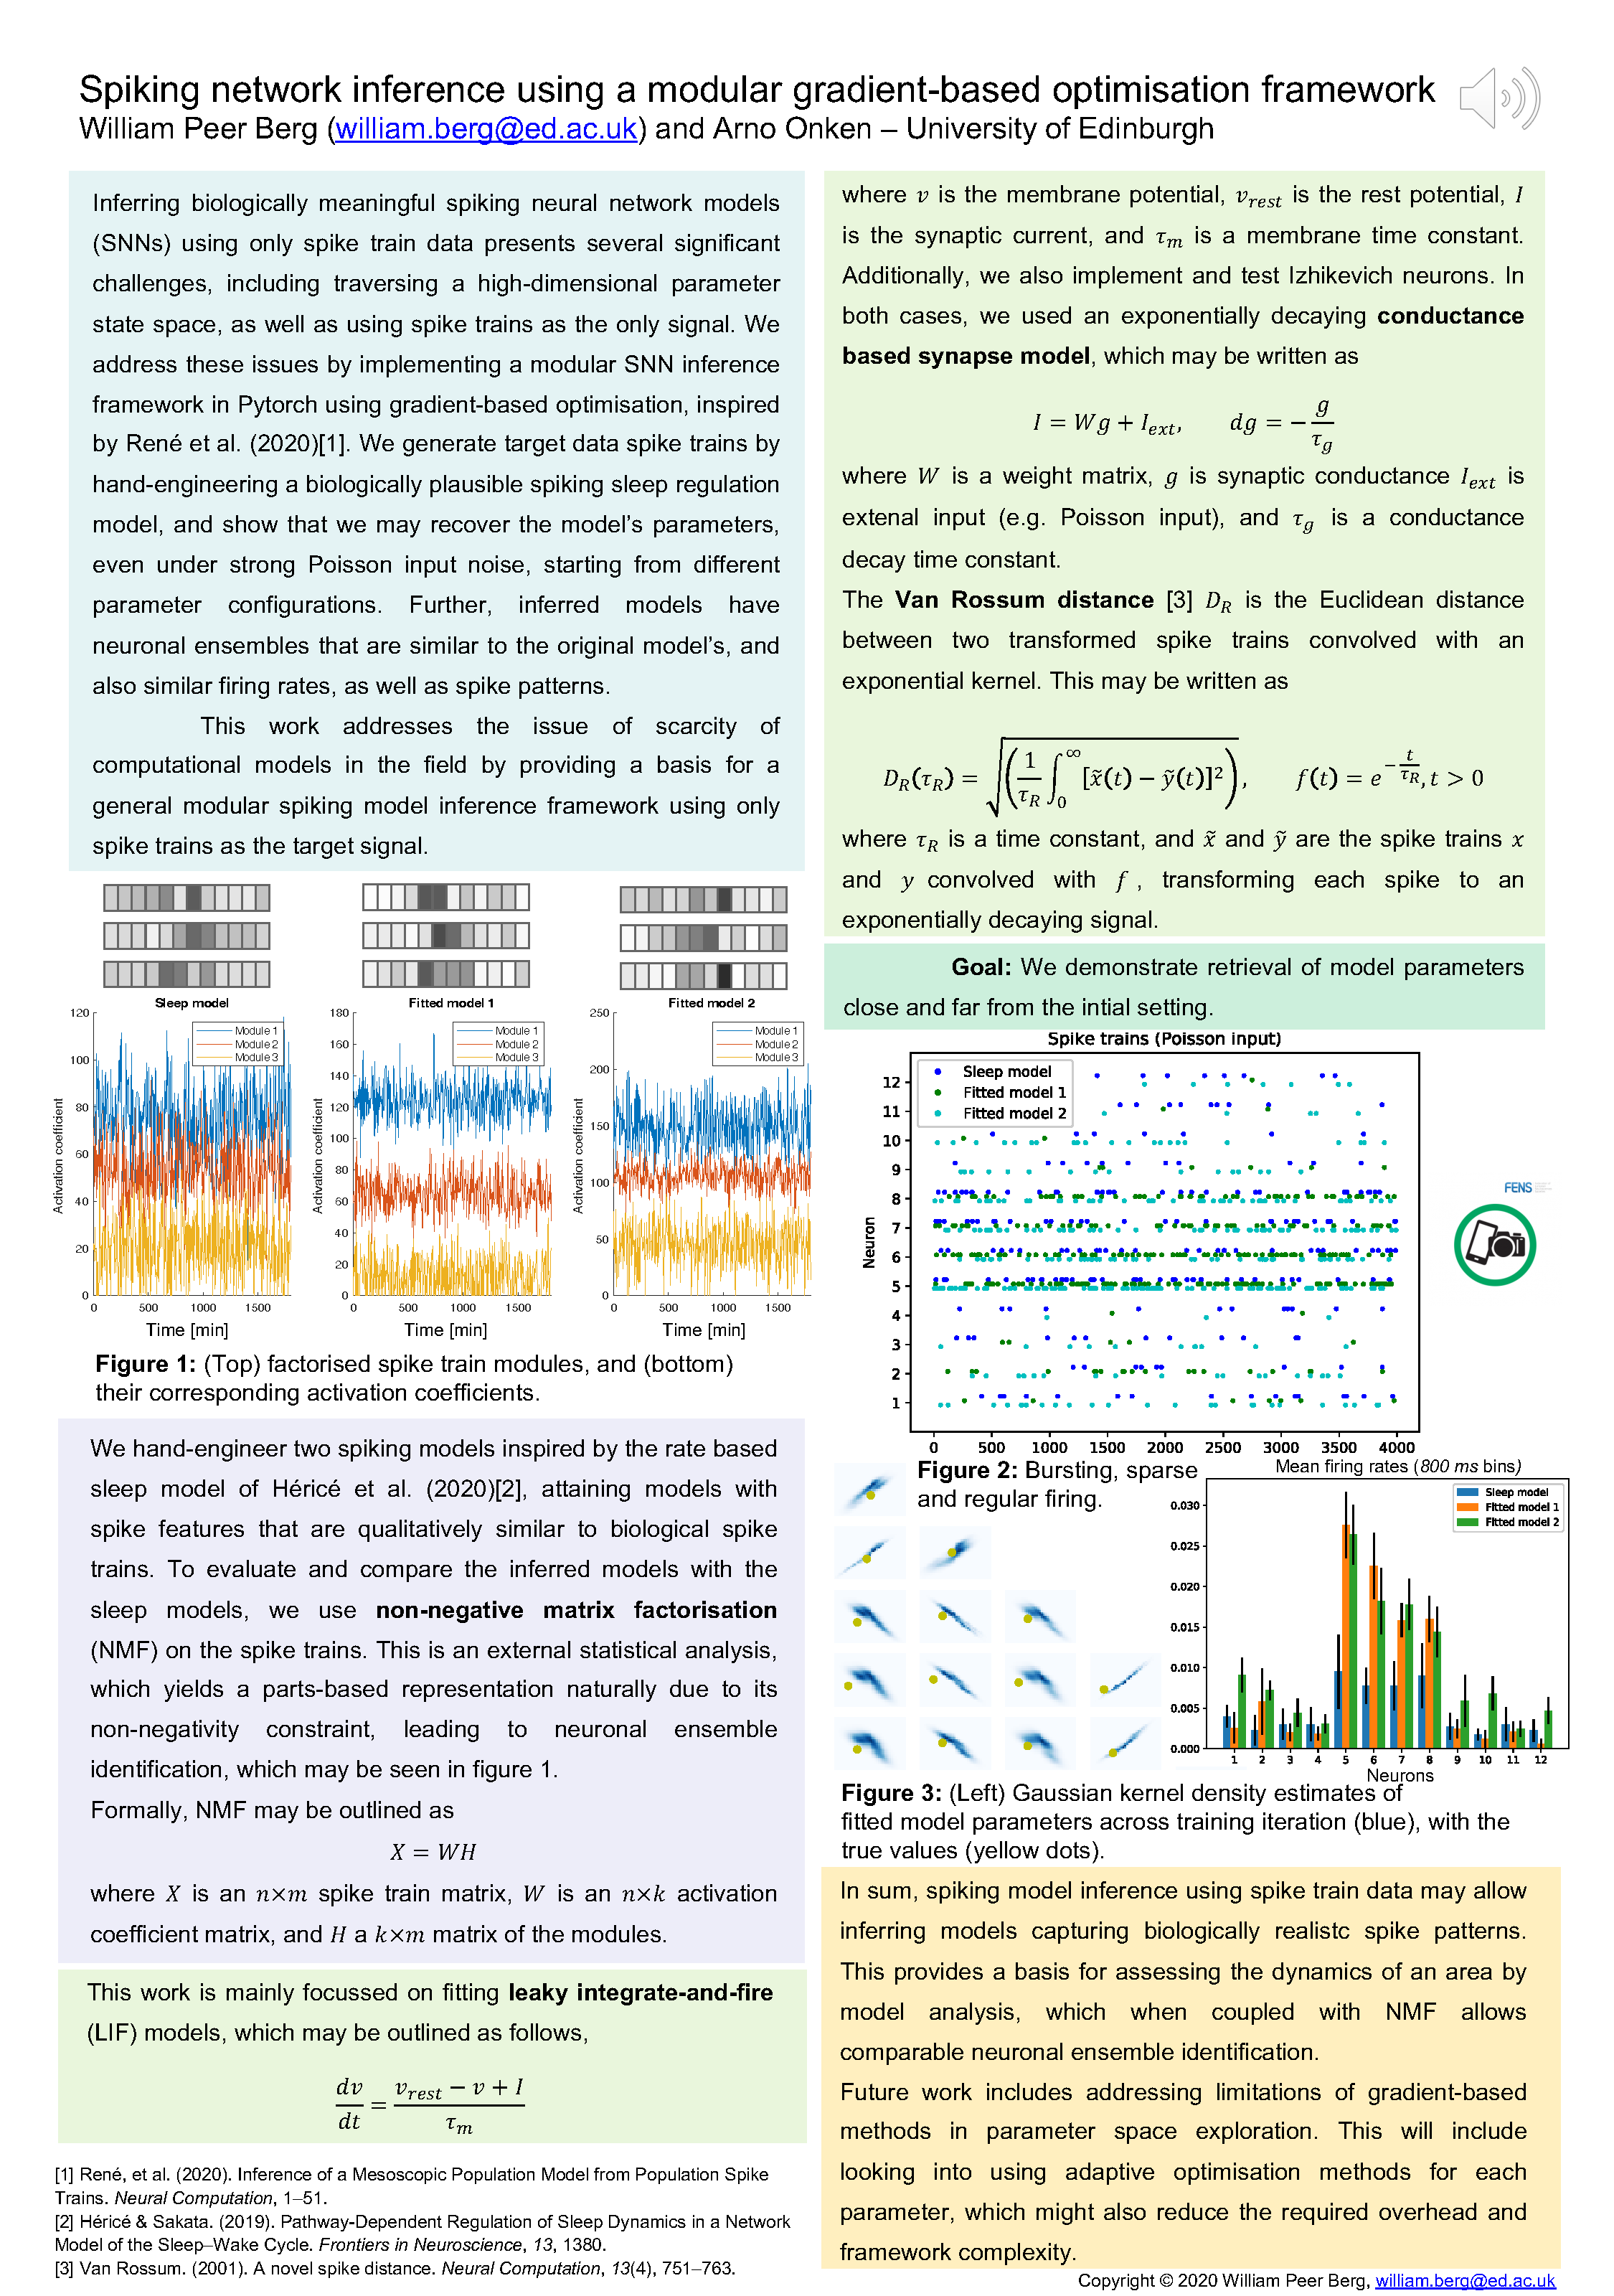
\includepdf[pages=-]{files/FENS-virtual-2020-e-Poster-W-P-Berg-and-A-Onken-Spiking-Network-Inference-Using-Gradient-Based-Optimisation-PORTRAIT-5.pdf}

\section{Report/paper draft: \textit{Parallel spiking neural network parameter inference using gradient based optimization}}
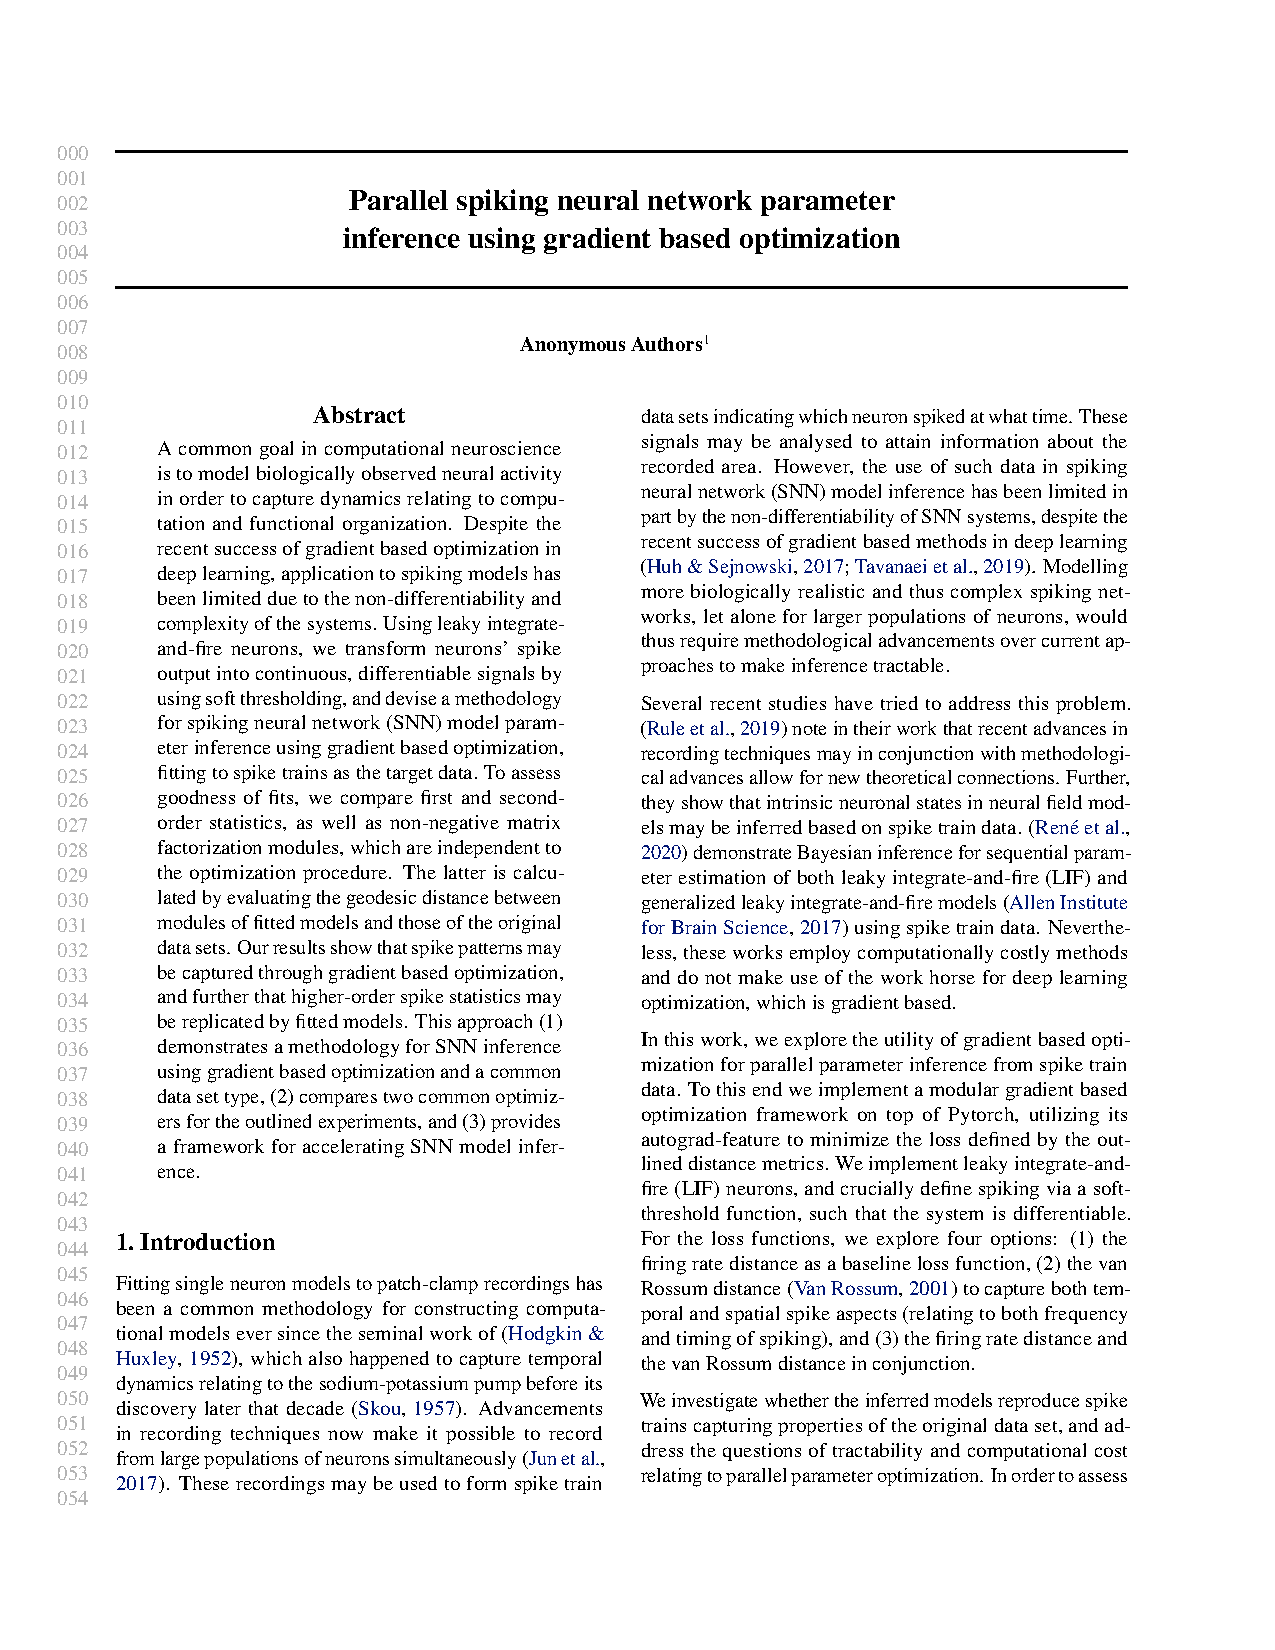
\includepdf[pages=-]{files/icml2021_draft_snn_inference.pdf}


% =======================================================
\chapter{Exact models with continuous spike signals}

Non-leaky integrate-and-fire (NLIF) model with subthreshold continuous spike signals defined to sum to 1 inside of an active zone \cite{Huh2017}.
% With NIF neurons, one could analytically show/solve the systems and show where noise would render the loss function useless. However, unsure how to test this for spike output task. Could we use (Mostafa, 2018) combined with (Huh \& Sejnowski, 2017)? Or at least the latter?

\subsection{Gated sub-threshold spike-signal model}

\subsection{Contribution: NLIF work}

analog output - discrete pulses, and internal states
research has been impeded by lack of supervised learning algorithms
they present differentiable formulation of SNNs, with exact gradient calculation
simple tasks
rate-based models fail to describe fast dynamics of spike-based computation
difficult to optimise discrete, binary all-or-none signals
other methods circumvent non-differentiability

"Note that the gradient calculation procedure involves multiplication between the presynaptic input source and the postsynaptic adjoint state pv, which is driven by the g ˙ps term: i.e. the product of postsynaptic spike activity and temporal difference of error. This is analogous to reward-modulated spike-time dependent plasticity (STDP) [17]."


% =======================================================
\chapter{Sleep regulation in the rodent brainstem}

My initial research proposal outlines a research project where the goal is to meet research needs within the field of sleep regulation through computational modelling.
More specifically, the aspiration was to model neurons of the pedunculopontine and laterodorsal tegmental areas within the brainstem during different brain states, based on their neuroanatomy as described, even though scarcely, within the literature, and based on in vivo data from these brain areas \cite{Herice2019c, Tsunematsu2019, Pal2007, Martinez-Gonzalez2011, Fraigne2015}.
Further, an overarching research goal was to be able to capture the emergence of neural ensembles as identified in vivo in the model by using non-negative matrix factorisation (NMF) \cite{Seung1999, Seung2001, Onken2016a}.
Computational modelling and spiking neural network (SNN) inference covers several research needs within the field of sleep research and the synthesis of neuroscience and its computational counterpart in that it addresses model scarcity, as well as a methodology for accelerating modelling by inference through gradient-based optimisation \cite{Herice2019c, Huh2017, Taherkhani2020}.
This was the foundation for sparking my interest in a methodological project in which we seek to automate biologically relevant neural network model inference, and more specifically to research both (1) the current state-of-the-art on SNN inference, and (2) leveraging ML based methods of gradient descent and optimisation for SNN inference \cite{Huh2017, Mostafa2020, Tavanaei2019b, Lee2016}.


\section{Modelling sleep regulation in the brainstem}

Sleep is widespread across different animal species, crucial to mental functioning. However, why we sleep, and how we sleep, remains to be understood. Some models exist that seek to capture the phasic nature of sleep, but mostly at an abstract level. There is as such a need for detailed models in the field, with no current models encompassing direct biological parallels. Addressing the need for modelling in the field, and seeking to illuminate how we sleep, we propose to use a set of recently combined methodologies that allow us to infer the most probable neuron-level spiking models based on only partial information, and partial neuronal recording data. In other words, the methodology allows for incorporating both existing knowledge, and to use spike sorted LFP recordings to infer the most statistically probable distributions of model parameters.

More specifically, using spike sorted data recorded from the mouse brain stem in the pedunculopontine and laterodorsal tegmental (PPT/LDT) areas, we address whether these areas do in fact initiate sleep stages, which has been previously hypothesised and recently debated. 
To address this, we looked at the temporal relationship between future and past state prediction, using linear discriminant analysis (LDA) on derived functional modules using non-negative matrix factorisation (NMF), replicating and extending the work reported by the collaborative lab from whom we have been granted access to the spike data.

Further, we study methodologies for inferring meaningful computational models using spike train data, and how they inferred models may be studied to evaluate the nature of the neurons by drawing upon the biology corresponding to their parameters within the literature.
This algorithmic approach applied to spike train data has, to the best of my knowledge, not been previously explored. This is due to the high dimensional parameter search space, which requires a correspondingly complex approach in order to make computation tractable.
As such, not only could an inferred model be used to address hypotheses such as whether sleep regulation within this area is mediated by an ensemble of cholinergic neurons, but the methodology could further be applied in other domains, using data of the same nature from different brain regions.
The approach requires only partial data - as is always a constraint within neuroscientific recordings. Using a form of Bayesian inference, measures of deviation and confidence may be defined comparatively between synthetic models and data, and the recorded spike trains considered as ‘ground truth’. Probable fits with a fair variance suggest meaningful inferred model parameter distributions. However, model quality metrics depend on the data for which the comparison is computed.

In more detail, the model inference method is based on modelling the probability of spiking for a neuron as a Bernoulli random variable, with the variable modelling spiking in each time bin. We construct time bins for the spike trains such that the probability of spiking in one bin may be approximately dependent only on the previous bin (which might be justified considering its refractory and synaptic time constants). This allows us to formulate the probability of a spike train as a Markov chain, and enables us to estimate population model parameters. Interestingly, the authors found that a better fit for a microscopic model was inferred when first performing gradient descent for a mesoscopic level model, representing each population with average parameters. 
This may be due to that inferring only one average parameter value per population regularises the training procedure by averaging over the parameter space of a microscopic model. 
There are two key points that I would like to communicate associated with that observation; (1) is that the complexity associated with the parameter space of microscopic models might make convergence towards a global optimum unlikely, and (2) that an average parameter might lose values that are of a secondary or tertiary order of importance, despite prominent in the data set, if somewhat conflicting with the final inferred average value. Addressing (2), it might be fruitful to allow for sets of average values for population models, investigating whether this might increase resulting microscopic model performance. Note that inference of the maximum a posteriori for corresponding microscopic models then might increase exponentially, or at least linearly, with the order of increased number of values inferred at the mesoscopic level. However, it might make sense to infer one average per neuron type as the population level, i.e. if it is believed that it contains for instance two sets of neuron types, or functional ensembles, such as inhibitory-excitatory neurons. This has to my knowledge not been attempted within this methodological approach.
Once a mesoscopic model has been attained, it may be used to synthetically generate data for use in the inference of a more detailed neuron-level or microscopic model. By generating synthetic data we may employ the family of Monte-Carlo (MC) methods. In order to accelerate convergence for computational efficiency, Hamiltonian MC is employed. This allows for approximating the full posterior over the most likely parameter distributions for microscopic models.

Statistically, model soundness may be considered in terms of comparison to a validation set stemming from the same experiment, and also across the 7 performed experiments. However, due to the nature of neuroscientific recordings, where there is a significant uncertainty in both the areas targeted with the silicon probes, and not the least due to significant individual differences for neural ensembles, it is unlikely that we can see neuron-level similarities across experiments. However, similarities at a population and functional level may occur if the same areas are recorded.

% Currently, the project is a work in progress, with implementation of the model and a corresponding gradient descent (GD) as well as HMC being in focus. GD may be partially implemented using the Theano library, as well as open-sourced modules, and HMC using the PyMC3 library.
% In order to finalise the implementation, there is a substantial amount of programming required, followed by an ever greater extent of testing, debugging, verification. Finally, when satisfied with the aforementioned, we may proceed to run experiments, analysing the results, and depending on the outcomes pursue further work.



\section{Neuroscience background}

\subsection{Sleep stages}
Three-process switch model. Different timescales may be at play, and constitute the switching-mechanism.
Also, can a meso-model be used in the first step of creation of such a model?

\subsection{PPT/LDT}
PPT/LDT LFP data; most spiking during NREMS
(to consider: Little time spent in NREMS)
Want to primarily look at REMS: disinhibition of monoaminergic LC projections (prerequisite; Timofeev et al. (2017)) (shut off / inhibited in LC by GABA), 

PPT/LDT:
Cholinergic are REMS and wake
GABAergic; REMS, wake, or both
NREM?

Look at single-cell resolution connectivity? (e.g. Martinez-Gonzalez, Mena-Segovia)

Complex circuitry means a myriad of ppt/ldt inputs, some of which are poorly understood.
Could these somehow be reverse-engineered given the state and neural activity, classifying the neurons into types, which can tell us something about the pathways involved, and whether they’re “ON” or “OFF”?
Simple state-driven input as on/off per state to the ensembles should tell us something about each ensemble and its state-preference? If so, these can be identified, parameters compared and fixed, and then we could try to reconstruct the projections - perhaps using the model of Herice et al. (2018)


\section{Analysis of data}
Data from PPT/LDT area/brainstem. Evaluation and assessment through (rigorous) analysis and classification/prediction of brain state. Shows four well-qualified experiments for further analysis and bridging using the mesoscopic modelling approach.
Provides a solid bridge from the domain of experimental data to generating data using a simulated model that is derived from a good data foundation that we know is well-aligned with brain state.

Idea: “ultradian” process for synchronous/asynchronous activity -> nREM/REM, also should give rise to qualities during wakefulness (such as better brainstorming/creativity, or some types of productivity in “phases”/stages)

Idea: Cell types and model parameters that may be used in type classification from fitting data to GLIF models is lacking for the mouse brainstem in the Allen Brain project database.

\section{Inference}

\subsection{GBO}

\subsection{ABC}

\subsection{Comparison and conclusion}


\chapter{Why the brain does not do backpropagation}

Receptive fields very robust, but continuous perturbation results in changes, also in higher visual areas
Individual differences
The brain is “born with too many neurons” - naturally does pruning
“Some neurons and parameters are highly important, whereas others aren’t” - Fisher information spans an ellipse in parameter-space(?), can see that some aren’t that important
Q: Can we compute the Fisher information locally? Essentially, yes. Parameter importance. Can also go further and do mean field approximation. ML does something like this. Local heuristics can be used efficiently to remove many parameters in network without “interference”. Turns out many of related neurons may be pruned away too.
Brain neurons highly recurrently connected.
Q: How does the brain do things?
Synaptic conn in brain constrains what patterns are visible to neurons
Brain is a dyn cyst
Can compute manifolds in which the activity lives and moves
Functioning: “Carried out by movements along manifolds”
Activity is modulated by incoming activity, which manipulate manifolds


If the structure that allows acquisition of new knowledge, as well as new heuristics, is successfully implemented, the ever-changing heuristics may lead to an autonomous agent. 
However, successfully implementing the aforementioned is an engineering challenge we have yet to overcome. It is difficult to predict what such an algorithm would need to contain, as most applications of DNNs are very domain specific, and extremely or fully prone to catastrophic forgetting when trained on a new data set.
There is still a fundamental gap between general knowledge acquisition and the specialised kind we see within ML.


“Computationally, we now know that optimization of trajectories gives rise to elegant solutions for very complex motor tasks (Harris and Wolpert, 1998; Todorov and Jordan, 2002; Mordatch et al., 2012). We suggest that cost function optimization occurs much more generally in shaping the internal representations and processes used by the brain. Importantly, we also suggest that this requires the brain to have mechanisms for efficient credit assignment in multilayer and recurrent networks.” - Marblestone et al. (2016). Frontiers in Computational Neuroscience
And it doesn’t matter what specific configuration a network reaches, as long as it reaches “the bottom of the loss curve”, i.e. finds a good/satisfactory solution. → Optimal is any configuration solving the task at hand, and optimal is plural, and diverse. Optimal can be a frontier in high-dimensional space. In Bayesian inference Macke argued we may be able to trace this front by drawing shapes between samples forming probable combinations in parameter-space.

Can we say something about this Pareto-front with GD?
When sampling from full posterior dist from a SBI posterior we get realistic data - when independently sampling from marginals we get unrealistic data. Flaw in model, and in assuming parameter independence.

Both of these methodologies get at a reasonable frontier - however, learning in itself in the structures is something different, remaining a mystery.


If only the temporal unfolding of spike events was done according to linear transformations, or in a ...
It may be argued that under similar conditions, we may detect things such as spike correlations and phase-locking, which may indicate a clear function of the timing of spiking in information processing - however, it is difficult to design a loss metric that would well capture this in a differentiable manner.
By correlation and number of mutations of the ordered spike train set, we can get closer to this - but such a metric would not be differentiable, nor would even such a metric be able to precisely measure whether one network is functionally equivalent to another.
Part of the difficulty stems from that (1) there are multiple configurations which can produce similar spike patterns, and thus we may hypothesise that there is no "ground-truth" optimal solution per se, and (2) due to the multiple factors of stochasticity we cannot operate with precise spike train comparisons. These two points result in that currently the way of going about to analyse biologically realistic models are closer to the way we analyse recordings from the biological brain. As such, a bridge between inference methodologies such as the ones successfully employed in ML, and the field of computational modelling is needed.




\bibliographystyle{plain}
\bibliography{references}

%% You can include appendices like this:
% \appendix
% 
% \chapter{First appendix}
% 
% \section{First section}
% 
% Markers do not have to consider appendices. Make sure that your contributions
% are made clear in the main body of the dissertation (within the page limit).

\end{document}
